\documentclass[a4paper]{article}
\usepackage[utf8]{inputenc} % para poder usar tildes en archivos UTF-8
\usepackage[spanish]{babel} % para que comandos como \today den el resultado en castellano
\usepackage{a4wide} % márgenes un poco más anchos que lo usual
\usepackage[showRevisiones]{caratula}
\usepackage{xcolor}
\usepackage{listings}
\lstset{basicstyle=\ttfamily,
  showstringspaces=false,
  commentstyle=\color{red},
  keywordstyle=\color{blue}
}

\begin{document}

\materia{Organización de Computadoras 66.20}
\tipoapunte{Trabajo Práctico #1}

\fecha{\today}

\autor{Flórez Del Carpio, Christian}{91011}{chris.florez.d.c@gmail.com}
\autor{Montenegro, Josefina}{94289}{mariajosefina.mont@gmail.com}
\autor{Quino López, Julián}{94224}{julianquino2@gmail.com}

\revision{13/10/2017}{-}{Entrega primera versión del TP}
\maketitle

\begin{abstract}
El siguiente trabajo práctico tiene como objetivo familiarizarse con el conjunto de instrucciones MIPS y el concepto de ABI, para lograr dicho propósito se debe implementar la lógica de detección de palíndromos en assembly, entendiendo como palabras a aquellas compuestas por letras [A-Z], números [0-9], guiones bajos y medios, es decir, cualquier combinación posible de los anteriormente mencionados, tal como estaba enunciado en el TP0.
\end{abstract}


\section{Introducción}
Pueden haber tres escenarios posibles, el caso en el cual el usuario ingresa archivo de entrada y salida, el caso en el que se ingresa un archivo de entrada solamente y por último el caso donde se recibe el archivo de salida. En caso de no proporcionar un archivo de texto como entrada, se requerirá ingresar el stream por entrada standard. Si no se especifica un archivo de salida, se mostrarán los resultados por salida standard. Esto es igual a lo explicando en el TP0.


\section{Desarrollo}

Se desarrolló un programa C, desde el cual se invoca a la función palindrome escrita en assembly. Esta función recibe como parámetros los archivos de entrada/salida (si no se hubiesen proporcionado tales archivos se toman los streams de entrada/salida standard) y las cantidades ibytes y obytes, las cuales describen la unidad de transferencia para escribir en el buffer de entrada/salida, respectivamente. Cuando no son proporcionados estos valores, se toma por defecto el valor 1.

\subsection{Comandos para compilar y ejecutar el programa}

Se puede compilar el programa con el siguiente comando:

\begin{lstlisting}[language=bash]
  $ gcc -Wall -g -o tp1 isPalindrome.c isPalindrome.S
\end{lstlisting}


Y luego ejecutarlo con el comando:

\begin{lstlisting}[language=bash]
  $ ./tp0 -i input.txt -o output.txt -I ibytes -O obytes
\end{lstlisting}

En caso de sólo querer especificar el archivo de entrada, debe ejecutarse, por ejemplo, de la siguiente manera:

\begin{lstlisting}[language=bash]
  $ ./tp0 -i input.txt -o -
\end{lstlisting}

Análogamente si se quiere ingresar un archivo de salida:

\begin{lstlisting}[language=bash]
  $ ./tp0 -i - -o output.txt
\end{lstlisting}

Es decir que con un guión medio indicamos que no se proporcionará un archivo para entrada/salida, acorde a lo que indica el enunciado.

\subsection{Otros comandos}

Pueden utilizarse comandos tales como help y version, de la siguiente forma:

\begin{lstlisting}[language=bash]
  $ ./tp0 -h
\end{lstlisting}

\begin{lstlisting}[language=bash]
  $ ./tp0 -V
\end{lstlisting}

\subsection{Código fuente C}
\begin{lstlisting}[language=C]
#include <stdio.h>
#include <string.h>
#include <getopt.h>
#include <stdlib.h>
#include <errno.h>
#include <unistd.h>

#define ERROR -1
#define SALIDA_EXITOSA 0

int inputFileno;
int outputFileno;

extern int palindrome(int ifd, size_t ibytes, int ofd, size_t obytes);

int main(int argc, char *argv[]) {

    int option = 0;
    char *ibytes = NULL, *obytes = NULL;
    const char *short_opt = "i:o:hVI:O:";
    struct option long_opt[] = {
            {"version",    no_argument,       NULL, 'V'},
            {"help",       no_argument,       NULL, 'h'},
            {"input",      required_argument, NULL, 'i'},
            {"output",     required_argument, NULL, 'o'},
            {"ibuf-bytes", required_argument, NULL, 'I'},
            {"obuf-bytes", required_argument, NULL, 'O'},
            {NULL, 0,                         NULL, 0}
    };
    FILE *inputFile = NULL;
    FILE *outputFile = NULL;

    while ((option = getopt_long(argc, argv, short_opt, long_opt, NULL)) != -1) {
        switch (option) {
            case 'V':
                printf("TP #0 de la materia Organización de Computadoras \n");
                printf("Alumnos: \n");
                printf("	Flórez Del Carpio Christian\n	Montenegro Josefina \n	Quino Lopez Julian \n");
                return 0;
            case 'h':
                printf("Usage: \n");
                printf("	%s -h \n", argv[0]);
                printf("	%s -V \n", argv[0]);
                printf("	%s [options] \n", argv[0]);
                printf("Options: \n");
                printf("	-V, --version    Print version and quit. \n");
                printf("	-h, --help       Print this information. \n");
                printf("	-o, --output     Location of the output file. \n");
                printf("	-i, --input      Location of the input file. \n");
                printf("        -I, --ibuf-bytes Byte-count of the input buffer. \n");
                printf("        -O, --obuf-bytes Byte-count of the output buffer. \n");
                return 0;
            case 'i':
                inputFile = fopen(optarg, "r");
                if (inputFile == NULL) {
                    fprintf(stderr, "Error archivo entrada: %s\n", strerror(errno));
                }
                break;
            case 'o':
                // verifico si existe el archivo
                if (access(optarg, W_OK) != -1) {
                    outputFile = fopen(optarg, "w+");
                    if (outputFile == NULL) {
                        fprintf(stderr, "Error archivo salida: %s\n", strerror(errno));
                        return ERROR;
                    }
                }
                break;
            case 'I':
                ibytes = optarg;
                break;
            case 'O':
                obytes = optarg;
                break;
            default:
                // así está en el manual de getopt
                abort();
        }
    }

    if (inputFile == NULL) inputFile = stdin;

    if (outputFile == NULL) outputFile = stdout;

    if (ibytes == NULL) ibytes = "1";

    if (obytes == NULL) obytes = "1";

    inputFileno = fileno(inputFile);
    outputFileno = fileno(outputFile);
    palindrome(inputFileno, (size_t)atoi(ibytes), outputFileno, (size_t)atoi(obytes));

    if(inputFile != stdin){
    	if (fclose(inputFile) == EOF) {
			fprintf(stderr, "Error fclose: %s\n", strerror(errno));
			return ERROR;
		}
	}

    if(outputFile != stdout) {
        if (fclose(outputFile) == EOF) {
    		fprintf(stderr, "Error fclose: %s\n", strerror(errno));
    		return ERROR;
    	}
    }

    return SALIDA_EXITOSA;
}
\end{lstlisting}

\subsection{Código fuente Assembly}
\begin{lstlisting}[language=Assembler]
#include <mips/regdef.h>
#include <sys/syscall.h>

#define MYMALLOC_SIGNATURE 0xdeadbeef

#ifndef PROT_READ
#define PROT_READ 0x01
#endif

#ifndef PROT_WRITE
#define PROT_WRITE 0x02
#endif

#ifndef MAP_PRIVATE
#define MAP_PRIVATE 0x02
#endif

#ifndef MAP_ANON
#define MAP_ANON 0x1000
#endif

	#int llenarBufferEntrada(int archivoIn,char* bufferEntrada,int tamanioIn)
	.text
	.align	2
	.globl	llenarBufferEntrada
	.ent	llenarBufferEntrada
llenarBufferEntrada:
	.frame	$fp,32,ra
	.set	noreorder
	.cpload	t9
	.set	reorder

	subu	sp,sp,32
	.cprestore  16
	sw		$fp,20(sp)
	move	$fp,sp
	sw		ra,12($fp)

	sw		a0,24($fp)
	sw		a1,28($fp)
	sw		a2,32($fp)
	li		v0,SYS_read
	syscall

	#probamos si hay errores primero
	bne		a3, zero, ErrorllenarBufferEntra
	bgt		zero,v0, ErrorllenarBufferEntra
	b		salidallenarBufferEntrada
ErrorllenarBufferEntra:
	li		v0,-1
	li	v0, SYS_exit
	li	a0, 1
	syscall
salidallenarBufferEntrada:
	lw		ra,12($fp)
	lw		$fp, 20(sp)
	addu	sp, sp, 32
	j		ra
	.end	llenarBufferEntrada


	#int llenarBufferSalida(char *bufferSalida,int tamanioBufferSalida,char *cadena,int contadorDeBufferSalida)
	.text
	.align	2
	.globl	llenarBufferSalida
	.ent	llenarBufferSalida
llenarBufferSalida:
	.frame	$fp,48,ra
	.set	noreorder
	.cpload	t9
	.set	reorder

	subu	sp,sp,48
	.cprestore  16
	sw		$fp,20(sp)
	move	$fp,sp
	sw		ra,12($fp)

	sw		a0,24($fp)    	#bufferSalida
	sw		a1,28($fp)		#tamanioBufferSalida
	sw		a2,32($fp)		#cadena
	sw		a3,36($fp)		#contadorDeBufferSalida

	sw		s6,0($fp)
	sw		s7,4($fp)

	move	s6,a0	#buffersalida
	move 	s7,a2	#cadena

	sw		zero,40($fp)

	move	a0,s7
	jal 	mystrlen
	sw		v0,44($fp)


whileDeProcesamientoDeCaracter:

	lw		t0,40($fp)
	lw		t1,44($fp)
	bge		t0,t1,salirWhileProcesamientoDeCaracter

	lw		t0,36($fp)
	lw		t1,28($fp)
	bne		t0,t1,noEstallenoElBuffer

	li		v0,SYS_write
	lw		a0,outputFileno
	move	a1,s6
	lw		a2,28($fp)
	syscall

	#me fijo si hay error
	bne		a3, zero, ErrorllenarBufferSalida
	bgt		zero,v0, ErrorllenarBufferSalida
	sw		zero,36($fp)

	b		whileDeProcesamientoDeCaracter
noEstallenoElBuffer:
	lw		t0,40($fp)
	move	t1,s7
	addu	t0,t0,t1
	lbu		t1,(t0)

	lw		t0,36($fp)
	move	t2,s6
	addu	t2,t2,t0
	sb		t1,(t2)

	lw		t0,36($fp)
	addu	t0,t0,1
	sw		t0,36($fp)

	lw		t0,40($fp)
	addu	t0,t0,1
	sw		t0,40($fp)

	b		whileDeProcesamientoDeCaracter
salirWhileProcesamientoDeCaracter:
	lw		t0,36($fp)
	lw		t1,28($fp)
	bne		t0,t1,agregarSaltoDeLinea

	li		v0,SYS_write
	lw		a0,outputFileno
	move	a1,s6
	lw		a2,28($fp)
	syscall

	bne		a3, zero, ErrorllenarBufferSalida
	bgt		zero,v0, ErrorllenarBufferSalida

	sw		zero,36($fp)

agregarSaltoDeLinea:

	move 	t0,s6
	lw		t1,36($fp)
	addu	t0,t0,t1
	li		t1,10
	sb		t1,(t0)


	lw		t0,36($fp)
	addu	t0,t0,1

	move 	v0,t0
	b		salidallenarBufferSalida
ErrorllenarBufferSalida:
	li		v0,-1
	li	v0, SYS_exit
	li	a0, 1
	syscall
salidallenarBufferSalida:
	lw		ra,12($fp)
	lw		s6,0($fp)
	lw		s7,4($fp)
	lw		$fp, 20(sp)
	addu	sp, sp, 48
	j		ra
	.end	llenarBufferSalida




	#int palindrome(int ifd, size_t ibytes, int ofd, size_t obytes)
	.text
	.align	2
	.globl	palindrome
	.ent	palindrome
palindrome:
	.frame	$fp,80,ra
	.set	noreorder
	.cpload	t9
	.set	reorder

	subu	sp,sp,80
	.cprestore  16
	sw		$fp,20(sp)
	move	$fp,sp

	sw		ra,12($fp)
	sw		a0,24($fp)
	sw		a1,28($fp)
	sw		a2,32($fp)
	sw		a3,36($fp)



	move 	a0,a1
	jal		mymalloc
	sw		v0,0($fp)
	move 	s0,v0			#guardo en s0 el buffer de entrada

	move 	a0,a3
	jal		mymalloc
	sw		v0,4($fp)
	move 	s1,v0			#guardo el buffer de salida

	li		t0,1
	sw		t0,64($fp) 		#variable para indicar la salida del Procesamiento

	sw		zero,48($fp)	#cantcaracteres
	move	s2,zero			#cadenaDeCaracteres
	sw		zero,52($fp)	#contadorDeBufferSalida

whilePrincipal:
	lw		t0,64($fp)
	li		t1,1
	bne 	t0,t1,salirwhilePrincipal

	lw		a0,inputFileno
	move	a1,s0
	lw		a2,28($fp)
	jal		llenarBufferEntrada
	sw		v0,40($fp)

	bne		v0,zero,seguir1
	sw		zero,64($fp)
seguir1:
	sw		zero,44($fp)

whileProcesadorBufferEntrada:
	lw		t0,44($fp)
	lw		t1,40($fp)
	bge		t0,t1,whilePrincipal
	ble		t1,zero,whilePrincipal

	lw		t0,48($fp)
	addu	t0,t0,1
	sw		t0,48($fp)

	move	t0,s0
	lw		t1,44($fp)
	addu	t0,t0,t1
	lb		t0,(t0)

	move	a0,s2
	move	a1,t0
	lw		a2,48($fp)
	jal		agregarCaracter
	move	s2,v0

	move	a0,s2
	lw		a1,48($fp)
	jal		seFormoUnaPalabra
	li		t0,1
	bne		t0,v0,NoseFormoPalabra

	lw		t0,48($fp)
	addu	t0,s2,t0
	sb		zero,-1(t0)

	move 	a0,s2
	jal		palindromo
	li		t0,1
	bne		v0,t0,inicializarValoresYbuffer

	move	a0,s1
	lw		a1,36($fp)
	move 	a2,s2
	lw		a3,52($fp)
	jal		llenarBufferSalida
	sw		v0,52($fp)

	b 		inicializarValoresYbuffer
NoseFormoPalabra:

	move	a0,s2
	lw		a1,48($fp)
	jal		seFormoUnaPalabra
	li		t0,2
	bne		t0,v0,seguir2


inicializarValoresYbuffer:
	move 	a0,s2
	jal		myfree
	sw		zero,48($fp)
	move	s2,zero

seguir2:
	lw		t0,44($fp)
	addu	t0,t0,1
	sw		t0,44($fp)

	b		whileProcesadorBufferEntrada

salirwhilePrincipal:
	li		v0,SYS_write
	lw		a0,outputFileno
	move	a1,s1
	lw		a2,52($fp)
	syscall
	bne		a3, zero, ErrorWrite
	bgt		zero,v0, ErrorWrite

	move 	a0,s0
	jal 	myfree
	b		salidaPalindrome
ErrorWrite:
	li		v0,-1
	li	v0, SYS_exit
	li	a0, 1
	syscall
salidaPalindrome:
	lw		ra,12($fp)
	lw		$fp, 20(sp)
	addu	sp, sp, 80
	j		ra
	.end	palindrome








	#int seFormoUnaPalabra(char *cadena,int cantidadCaracteres)
	.text						#retorna 1 si se formo la palbra
	.align	2					#retirna 2 se lleno el buffer con un solo caracter invalido
	.globl	seFormoUnaPalabra	#retorna 0 si no se formo la palabra
	.ent	seFormoUnaPalabra
seFormoUnaPalabra:
	.frame	$fp,20,ra
	.set	noreorder
	.cpload	t9
	.set	reorder
	subu	sp,sp,20
	.cprestore 16
	sw		$fp,20(sp)
	move 	$fp,sp
	sw		ra,12($fp)

	sw		a0,0($fp)
	sw		a1,4($fp)

	addu	v0,a1,a0
	lbu		t0,-1(v0)
	sll		t0,t0,24
	sra		t0,t0,24
	sw		t0,8($fp)

	move	a0,t0
	jal		validCharacter

	move	t0,zero
	bne		t0,v0,noseFormoLaPalabra
	addu	t0,zero,1
	lw		t1,4($fp)
	beq		t1,t0,bufferVacio
	addu	v0,zero,1
	b		SalirSeFormoUnaPalabra
bufferVacio:
	move 	v0,zero
	addu 	v0,v0,2
	b		SalirSeFormoUnaPalabra
noseFormoLaPalabra:
	move v0,zero

SalirSeFormoUnaPalabra:
	lw 		ra,12($fp)
	lw		$fp, 20(sp)
	addu	sp, sp, 20
	j 		ra
	.end	seFormoUnaPalabra






	#int validCharacter(char character), 1 si es valido y 0 si es invalido
	.text
	.align	2
	.globl	validCharacter
	.ent	validCharacter
validCharacter:
	.frame	$fp,20,ra
	.set	noreorder
	.cpload	t9
	.set	reorder
	subu	sp,sp,20
	.cprestore 16
	sw		$fp,20(sp)
	move 	$fp,sp
	sw		ra,12($fp)

	sw		a0,0($fp);
	sll		a0,a0,24
	sra		a0,a0,24

	#aca valido los numero
	li		t0,57
	ble		a0,	t0,validesDeNumeros
	b		verMayuscula
validesDeNumeros:
	li		t0,48
	bge		a0,t0, salidaValida

verMayuscula:
	#valido palabras mayusculas
	li		t0,90
	ble		a0,	t0,validesMayusculas
	b		verMinuscula
validesMayusculas:
	li		t0,65
	bge		a0,t0, salidaValida

verMinuscula:
	#valido palabras minusculas
	li		t0,122
	ble		a0,	t0,validesMinusculas
	b		verOtrosCaracteres
validesMinusculas:
	li		t0,97
	bge		a0,t0, salidaValida

verOtrosCaracteres:
	#guion
	li		t0,45
	beq		a0,t0,salidaValida

	#guion bajo
	li		t0,95
	beq		a0,t0,salidaValida
salidaInvalida:
	move 	v0,zero
	b		SalirValidCharacter
salidaValida:
	move 	v0,zero
	addu	v0,v0,1

SalirValidCharacter:
	lw 		ra,12($fp)
	lw		$fp, 20(sp)
	addu	sp, sp, 20
	j 		ra
	.end	validCharacter


	#char* agregarCaracter(char* cadena,char caracterExtradido,int cantCaracteres)
	.text
	.align	2
	.globl	agregarCaracter
	.ent	agregarCaracter
agregarCaracter:
	.frame	$fp,48,ra
	.set	noreorder
	.cpload	t9
	.set	reorder
	subu	sp,sp,48
	.cprestore 16
	sw		$fp,48(sp)
	move 	$fp,sp
	sw		ra,12($fp)

	sw		s0,24($fp)
	sw		s1,28($fp)
	sw		s2,32($fp)
	sw		s3,36($fp)
	move	s3,a0
	move	s1,a2
	sll		a1,a1,24
	sra		s2,a1,24
	move	a0,a2
	jal		mymalloc

	move	s0,v0
	beq		s3,zero,incertarCaracter

	move	a0,v0
	move	a1,s3
	move	a2,s1
	jal		mystrlcpy

incertarCaracter:
	addu	v0,s0,s1
	sb		s2,-1(v0)
	move	v0,s0

	lw		ra,12($fp)
	lw		s0,24($fp)
	lw		s1,28($fp)
	lw		s2,32($fp)
	lw		s3,36($fp)

	lw		$fp,48($fp)
	addu	sp,sp,48
	j	ra
	.end	agregarCaracter



	#int palindromo(char *palabra)
	.text
	.align	2					#devulve 1 si es palindrome
	.globl	palindromo			#devulve 0 si no lo son
	.ent	palindromo
palindromo:
	.frame	$fp,24,ra
	.set	noreorder
	.cpload	t9
	.set	reorder

	subu	sp,sp,24

	.cprestore  16
	sw		$fp,20(sp)
	move	$fp,sp
	sw		ra,12($fp)
	sw		a0, 0($fp)

	jal		mystrlen
	addu	t0,zero,1
	beq		t0,v0,esPalindromo

	lw		a0,0($fp)
	jal		transformarMinuscula
	sw		v0,24($fp)

	lw 		a0,24($fp)
	jal 	invertirPalabra
	sw		v0,4($fp)
	lw 		a0, 24($fp)
	lw 		a1, 4($fp)
	jal		palabrasIguales
	addu	t0,zero,1
	beq		v0,t0,esPalindromo
	b 		noEsPalindromo
esPalindromo:
	addu v0,zero,1				#devulve 1 si es palindromo
	b 		salirPalindromo
noEsPalindromo:
	move v0,zero				#devuelve cero si no es palindromo
salirPalindromo:
	lw 		ra,12($fp)
	lw		$fp, 20(sp)
	addu	sp, sp, 24
	j 		ra
	.end	palindromo


	#char* transformarMinuscula(char* cadena)
	.text
	.align	2
	.globl	transformarMinuscula
	.ent	transformarMinuscula
transformarMinuscula:
	.frame	$fp,40,ra
	.set	noreorder
	.cpload	t9
	.set	reorder

	subu	sp,sp,40

	.cprestore  16
	sw		$fp,20(sp)
	move	$fp,sp
	sw		ra,12($fp)
	sw		a0, 24($fp)

	lw 		a0, 24($fp)
	jal		mystrlen
	sw 		v0, 0($fp) 		#guardo la cantidad de palabras
	beq 	v0,zero,palabraVacia
	move 	a0,v0
	addu 	a0,a0,1 		#sumo uno para el valor de \0
	jal 	mymalloc
	sw 		v0,28($fp) 		#guardo el puntero de la nueva palabra
	lw 		t1,24($fp)		#cargo la primera palabra para invetir
looptransformarMinuscula:
	lbu 	t2,0(t1)
	sll		t2,t2,24
	sra		t2,t2,24
	beq 	t2,zero,agregarfinDeVector

	#verificar si es mayucula
	li		t0,90
	ble		t2,	t0,verificarMayusculas
	b		cargarCaracter
verificarMayusculas:
	li		t0,65
	bge		t2,t0, esMayucula
	b		cargarCaracter
esMayucula:
	addu	t2,t2,32
cargarCaracter:
	sb 		t2,0(v0)
	addu 	t1,t1,1 			#sumo en uno la posicion de la primera palabra
	addu 	v0,v0,1 			#resto uno a la posicion de la segunda palabra
	b 		looptransformarMinuscula
agregarfinDeVector:
	lw 		v0,28($fp)		#obntengo de nuevo la dereccion inicial
	lw 		t0,0($fp)
	addu 	v0,v0,t0		#me muevo a la ultima posicion del vector
	sb 		zero,0(v0)		#copio el nulo en la ultima posicion
	lw 		v0,28($fp)
	b 		salirtransformarMinuscula
palabraVacia:
	move 	v0,zero
salirtransformarMinuscula:
	lw 		ra,12($fp)
	lw		$fp, 20(sp)
	addu	sp, sp, 40
	j 		ra
	.end	transformarMinuscula


	.text
	.align	2
	.globl	invertirPalabra
	.ent	invertirPalabra
invertirPalabra:
	.frame	$fp,40,ra
	.set	noreorder
	.cpload	t9
	.set	reorder

	subu	sp,sp,40

	.cprestore  16
	sw		$fp,20(sp)
	move	$fp,sp
	sw		ra,12($fp)
	sw		a0, 24($fp)

	lw 		a0, 24($fp)
	jal		mystrlen
	sw 		v0, 0($fp) 		#guardo la cantidad de palabras
	beq 	v0,zero,vacio
	move 	a0,v0
	addu 	a0,a0,1 		#sumo uno para el valor de \0
	jal 	mymalloc 		#cada ver el valor de retorno para poder salir si hay error
	sw 		v0,28($fp) 		#guardo el puntero de la nueva palabra
	lw 		t0, 0($fp) 		# t0 tiene el tamanio de la palabra
	subu 	t0,t0,1			#resto uno para q sea la posicion
	addu 	v0,v0,t0 		#este es la posicion del caracter a cipiar
	lw 		t1,24($fp)		#cargo la primera palabra para invetir

loopInvertirPalabra:
	lbu 	t2,0(t1)
	beq 	t2,zero,procesarSalida
	sb 		t2,0(v0) 		#t2 tiene un caracter y lo copio

	addu t1,t1,1 			#sumo en uno la posicion de la primera palabra
	subu v0,v0,1 			#resto uno a la posicion de la segunda palabra
	b loopInvertirPalabra
procesarSalida:
	lw 		v0,28($fp)		#obntengo de nuevo la dereccion inicial
	lw 		t0,0($fp)
	addu 	v0,v0,t0		#me muevo a la ultima posicion del vector
	sb 		zero,0(v0)		#copio el nulo en la ultima posicion
	lw 		v0,28($fp)		#restauro el v0 en la posicion incial para ser devuelto
	b 		salirInvertirPalabra
vacio:
	move 	v0,zero
salirInvertirPalabra:
	lw 		ra,12($fp)
	lw		$fp, 20(sp)
	addu	sp, sp, 40
	j 		ra
	.end	invertirPalabra


	.text
	.align	2
	.globl	palabrasIguales
	.ent	palabrasIguales
palabrasIguales:
	.frame	$fp,40,ra
	.set	noreorder
	.cpload	t9
	.set	reorder

	subu	sp,sp,40

	.cprestore  16
	sw		$fp,20(sp)
	move	$fp,sp
	sw		ra,12($fp)
	sw		a0, 24($fp)
	sw		a1, 28($fp)


	lw 		a0, 24($fp)
	jal		mystrlen
	sw 		v0, 32($fp)

	lw 		a0, 28($fp)
	jal		mystrlen
	sw 		v0, 36($fp)

	lw t0, 	32($fp)
	lw t1, 	36($fp)
	beq 	t0,t1, igualesTamanio
	b		noIguales

igualesTamanio:
	lw 		t0,24($fp)		#direccion al primera caracter de la primera palabra
	lw 		t1,28($fp)		#direccion al primera caracter de la segunda palabra
	lw 		t2,32($fp)		#tamanio de la palabra (tienen el mismo tamanio los dos)
	move 	t3,zero			#contador (empieza desde el cero)
loopPalabrasIguales:

	lbu		v0,0(t0)		#cargo el primer caracter en v0
	lbu		v1,0(t1)

	beq		v0,zero,iguales	#cuando llego al final de la palabra
	bne 	v0,v1,noIguales

	addu	t0,t0,1			#t0++
	addu	t1,t1,1			#t1++

	b 		loopPalabrasIguales
iguales:
	addu	v0,zero,1
	b 		salirPalabrasIguales
noIguales:
	move 	v0,zero
salirPalabrasIguales:
	lw 	ra,12($fp)
	lw	$fp, 20(sp)
	addu	sp, sp, 40
	j 	ra
	.end	palabrasIguales


	.text
	.align	2
	.globl	mystrlen
	.ent	mystrlen
mystrlen:
	.frame	$fp, 16, ra
	.set	noreorder
	.cpload	t9
	.set	reorder
	subu	sp, sp, 16
	.cprestore 0
	sw		gp, 4(sp)
	sw		$fp, 8(sp)
	move	$fp, sp
	sw		a0, 16(sp)

	li		v0, 0
mystrlenLoop:
	lb		t0, 0(a0)
	beqz	t0, mystrlenSalida
	addiu	a0, a0, 1
	addiu	v0, v0, 1
	j		mystrlenLoop

mystrlenSalida:
	lw		$fp, 8(sp)
	addu	sp, sp, 16
	j		ra
	.end	mystrlen


	.text
	.align	2
	.globl	mystrlcpy
	.ent	mystrlcpy
mystrlcpy:
	.frame	$fp,24,ra
	.set	noreorder
	.cpload	t9
	.set	reorder
	subu	sp,sp,24
	.cprestore  16

	sw		$fp,20(sp)
	move	$fp,sp
	sw		a0,24($fp)
	sw		a1,28($fp)
	sw		a2,32($fp)

	lw		t1,24($fp)
	sw		t1,0($fp)
	lw		t1,28($fp)
	sw		t1,4($fp)
	lw		t1,32($fp)
	sw		t1,8($fp)

	lw		t1,8($fp)
	beq		t1,zero,$N0		# si la cantidad de caracteres a copiar es cero salto a NO

$if1:
	lw		t2,8($fp)
	addu	t2,t2,-1
	sw		t2,8($fp)
	bne		t2,zero,tranferenciaDeCaracteres
	b		$N0

tranferenciaDeCaracteres:
	lw		a1,0($fp)
	lw		v1,4($fp)

	lbu		v0,0(v1)
	sb		v0,0(a1)

	lbu		v0,0(a1)

	addu	v1,v1,1
	addu	a1,a1,1
	sw		v1,4($fp)
	sw		a1,0($fp)

	sll		v0,v0,24
	sra		v0,v0,24

	bne		v0,zero,$if1

$N0:
	lw		t0,8($fp)
	bne		t0,zero,$Nnot0		# si la cantidad de caracteres es igual a cero


	lw		t0,32($fp)
	beq		t0,zero,$e_while

	lw		t0,0($fp)
	sb		zero,0(t0)

$e_while:

	lw		v0,4($fp)
	lbu		t0,0(v0)

	addu	v0,v0,1
	sw		v0,4($fp)

	sll		v0,t0,24
	sra		v0,v0,24
	bne		v0,zero,$e_while

$Nnot0:
	lw		v1,4($fp)
	lw		v0,28($fp)
	subu	v0,v1,v0
	addu	v0,v0,-1

	lw		$fp,20(sp)
	addu	sp,sp,24
	j		ra
	.end	mystrlcpy


	.text
	.align	2
	.globl	mymalloc
	.ent	mymalloc
mymalloc:
	subu	sp, sp, 56
	sw		ra, 48(sp)
	sw		$fp, 44(sp)
	sw		a0, 40(sp)  # Temporary: original allocation size.
	sw		a0, 36(sp)  # Temporary: actual allocation size.
	li		t0, -1
	sw		t0, 32(sp)  # Temporary: return value (defaults to -1).
#if 0
	sw		a0, 28(sp)  # Argument building area (#8?).
	sw		a0, 24(sp)  # Argument building area (#7?).
	sw		a0, 20(sp)  # Argument building area (#6).
	sw		a0, 16(sp)  # Argument building area (#5).
	sw		a0, 12(sp)  # Argument building area (#4, a3).
	sw		a0,  8(sp)  # Argument building area (#3, a2).
	sw		a0,  4(sp)  # Argument building area (#2, a1).
	sw		a0,  0(sp)  # Argument building area (#1, a0).
#endif
	move	$fp, sp

	# Adjust the original allocation size to a 4-byte boundary.
	#
	lw	t0, 40(sp)
	addiu	t0, t0, 3
	and	t0, t0, 0xfffffffc
	sw	t0, 40(sp)

	# Increment the allocation size by 12 units, in order to
	# make room for the allocation signature, block size and
	# trailer information.
	#
	lw	t0, 40(sp)
	addiu	t0, t0, 12
	sw	t0, 36(sp)

	# mmap(0, sz, PROT_READ|PROT_WRITE, MAP_PRIVATE|MAP_ANON, -1, 0)
	#
	li	v0, SYS_mmap
	li	a0, 0
	lw	a1, 36(sp)
	li	a2, PROT_READ|PROT_WRITE
	li	a3, MAP_PRIVATE|MAP_ANON

	# According to mmap(2), the file descriptor
	# must be specified as -1 when using MAP_ANON.
	#
	li	t0, -1
	sw	t0, 16(sp)

	# Use a trivial offset.
	#
	li	t0, 0
	sw	t0, 20(sp)

	# XXX TODO.
	#
	sw	zero, 24(sp)
	sw	zero, 28(sp)

	# Excecute the syscall, save the return value.
	#
	syscall
	sw	v0, 32(sp)
	beqz	v0, mymalloc_return

	# Success. Check out the allocated pointer.
	#
	lw	t0, 32(sp)
	li	t1, MYMALLOC_SIGNATURE
	sw	t1, 0(t0)

	# The actual allocation size goes right after the signature.
	#
	lw	t0, 32(sp)
	lw	t1, 36(sp)
	sw	t1,  4(t0)

	# Trailer information.
	#
	lw	t0, 36(sp) # t0: actual allocation size.
	lw	t1, 32(sp) # t1: Pointer.
	addu	t1, t1, t0 # t1 now points to the trailing 4-byte area.
	xor	t2, t0, MYMALLOC_SIGNATURE
	sw	t2, -4(t1)

	# Increment the result pointer.
	#
	lw	t0, 32(sp)
	addiu	t0, t0, 8
	sw	t0, 32(sp)

mymalloc_return:
	# Restore the return value.
	#
	lw	v0, 32(sp)

	# Destroy the stack frame.
	#
	move	sp, $fp
	lw	ra, 48(sp)
	lw	$fp, 44(sp)
	addu	sp, sp, 56

	j	ra
	.end	mymalloc

	.globl	myfree
	.ent	myfree
myfree:
	subu	sp, sp, 40
	sw	ra, 32(sp)
	sw	$fp, 28(sp)
	sw	a0, 24(sp)  # Temporary: argument pointer.
	sw	a0, 20(sp)  # Temporary: actual mmap(2) pointer.
	move	$fp, sp

	# Calculate the actual mmap(2) pointer.
	#
	lw	t0, 24(sp)
	subu	t0, t0, 8
	sw	t0, 20(sp)

	# XXX Sanity check: the argument pointer must be checked
	# in before we try to release the memory block.
	#
	# First, check the allocation signature.
	#
	lw	t0, 20(sp) # t0: actual mmap(2) pointer.
	lw	t1, 0(t0)
	bne	t1, MYMALLOC_SIGNATURE, myfree_die

	# Second, check the memory block trailer.
	#
	lw	t0, 20(sp) # t0: actual mmap(2) pointer.
	lw	t1, 4(t0)  # t1: actual mmap(2) block size.
	addu	t2, t0, t1 # t2: trailer pointer.
	lw	t3, -4(t2)
	xor	t3, t3, t1
	bne	t3, MYMALLOC_SIGNATURE, myfree_die

	# All checks passed. Try to free this memory area.
	#
	li	v0, SYS_munmap
	lw	a0, 20(sp) # a0: actual mmap(2) pointer.
	lw	a1, 4(a0)  # a1: actual allocation size.
	syscall

	# Bail out if we cannot unmap this memory block.
	#
	bnez	v0, myfree_die

	# Success.
	#
	j myfree_return

myfree_die:
	# Generate a segmentation fault by writing to the first
	# byte of the address space (a.k.a. the NULL pointer).
	#
	sw t0, 0(zero)

myfree_return:
	# Destroy the stack frame.
	#
	move	sp, $fp
	lw	ra, 32(sp)
	lw	$fp, 28(sp)
	addu	sp, sp, 40

	j	ra
	.end	myfree
	.rdata

error1:
	.ascii	"Error : %s\n\000"
aca:
	.ascii	"aca\n\0"

\end{lstlisting}

\section{Casos de prueba}

A continuación se muestran unos casos de prueba desde la consola del GXEmul, los textos utilizados se detallarán al final.


\begin{figure}[!htp]
\begin{center}
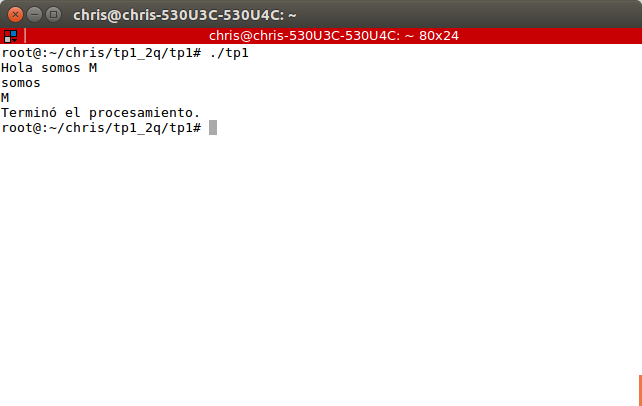
\includegraphics[width=0.5\textwidth]{imagenes_casosDePrueba_tp1/prueba0.png}
\caption{Prueba utilizando entrada y salida standard, y el tamaño en bytes por defecto del buffer de entrada y salida.} \label{fig001}
\end{center}
\end{figure}

\begin{figure}[!htp]
\begin{center}
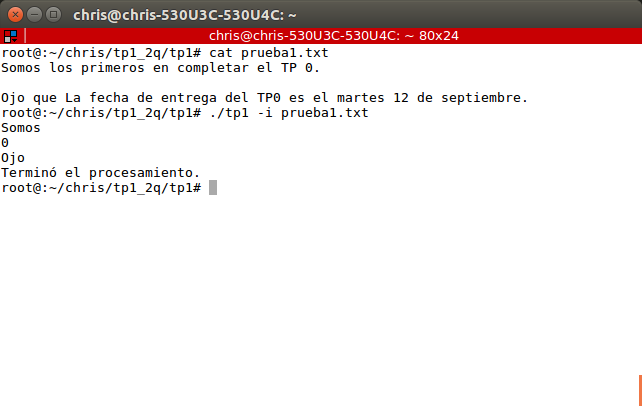
\includegraphics[width=0.5\textwidth]{imagenes_casosDePrueba_tp1/prueba_1archivoDeEntrada.png}
\caption{Prueba utilizando archivo de entrada y salida standard, y el tamaño en bytes por defecto del buffer de entrada y salida.} \label{fig001}
\end{center}
\end{figure}

\begin{figure}[!htp]
\begin{center}
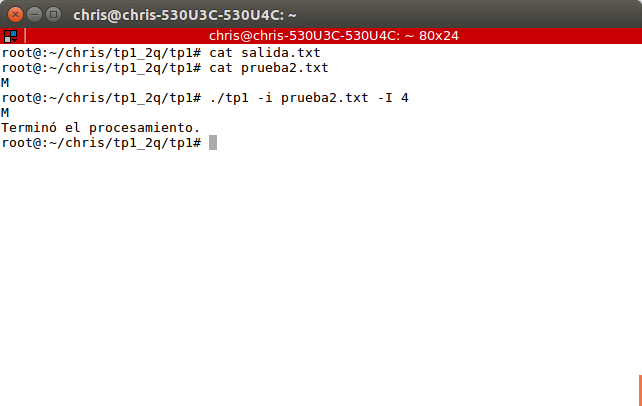
\includegraphics[width=0.5\textwidth]{imagenes_casosDePrueba_tp1/prueba2_entrada_4.png}
\caption{Prueba utilizando archivo de entrada especificando el tamaño del buffer de entrada y salida standard con tamaño de buffer de salida por defecto.} \label{fig001}
\end{center}
\end{figure}

\begin{figure}[!htp]
\begin{center}
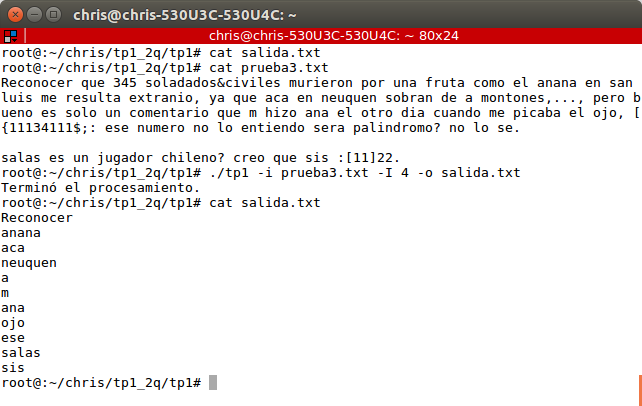
\includegraphics[width=0.5\textwidth]{imagenes_casosDePrueba_tp1/prueba3_archivoEntrada_4_salida_default.png}
\caption{Prueba utilizando otro archivo de entrada, especificando el tamaño de buffer de entrada, archivo de salida y tamaño de buffer de salida por defecto.} \label{fig001}
\end{center}
\end{figure}

\begin{figure}[!htp]
\begin{center}
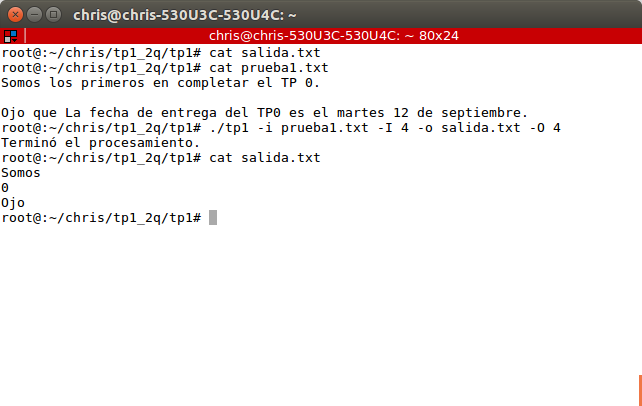
\includegraphics[width=0.5\textwidth]{imagenes_casosDePrueba_tp1/prueba1_archivoEntrada_4_salida_4.png}
\caption{Prueba utilizando archivo de entrada y salida, y especificando el tamaño del buffer de entrada y salida.} \label{fig001}
\end{center}
\end{figure}

\begin{figure}[!htp]
\begin{center}
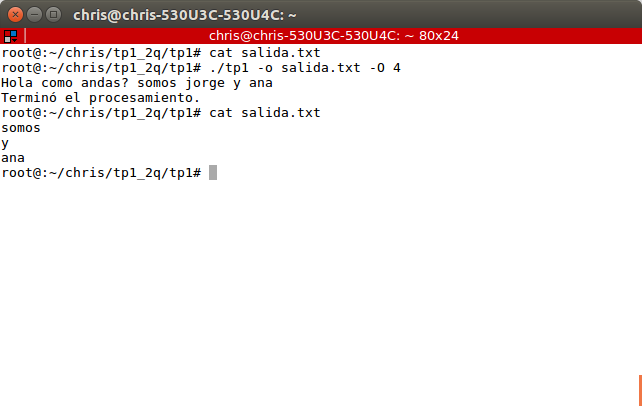
\includegraphics[width=0.5\textwidth]{imagenes_casosDePrueba_tp1/pruebaStdin_salida_4.png}
\caption{Prueba utilizando entrada standard y tamaño del buffer de entrada por defecto, archivo de salida y especificando tamaño de buffer de salida.} \label{fig001}
\end{center}
\end{figure}

\pagebreak
\subsection{Textos utilizados}

\paragraph{Prueba 1:}

Somos los primeros en completar el TP 0.

Ojo que La fecha de entrega del TP0 es el martes 12 de septiembre.

\paragraph{Prueba 2:}

M

\paragraph{Prueba 3:} 

Reconocer que 345 soladados&civiles murieron por una fruta como el anana en san luis me resulta extranio, ya que aca en neuquen sobran de a montones,..., pero bueno es solo un comentario que m hizo ana el otro dia cuando me picaba el ojo, [{11134111\$;: ese numero no lo entiendo sera palindromo? no lo se.

salas es un jugador chileno? creo que sis :[11]22.


\section{Código MIPS generado} 

\subsection{Código fuente Assembly}
\begin{lstlisting}[language=Assembler]
    
\end{lstlisting}


\section{Conclusiones}
El trabajo práctico nos resultó interesante, aprendimos a programar básicamente en assembly y a utilizar la convención de la ABI vista en clase. 

\begin{thebibliography}{1}

\bibitem{lib} GetOpt library, https://www.gnu.org/software/libc/manual/html_node/Example-of-Getopt.html.

\bibitem{stack} StackOverflow, https://www.stackoverflow.com.

\end{thebibliography}

\end{document}
